\chapter{Theory and methods}
\label{chap:theory}

Heat transfer is customarily described theoretically either at an atomistic level, monitoring the energy exchanged between individual atoms, or by treating the heat carriers as a gas of particles. While the latter particle picture is highly useful for, e.g., structures too large for atomic scale treatment, the structures considered in this thesis require atomic scale modeling to capture, e.g., the wave nature of energy carriers.

This chapter reviews the microscopic theory and computational methods used in the thesis. Sections \ref{sec:th_eom1} and \ref{sec:th_eom2} present the relevant equations governing phononic, electronic and photonic energy transfer in microscopic scale. To highlight the common features in the modeling of different carriers, we start by postulating the Langevin equations of motion for the three carriers in Sec. \ref{sec:th_eom1}. Carrier-specific details and the derivation of the presented linearized equations are presented in \ref{sec:th_eom2}. 

Langevin theory is used throughout the thesis to model thermal fluctuations and dissipation, and this theory and the fluctuation-dissipation theorem (FDT) are discussed in Sec. \ref{sec:th_langevin}. All calculations in the thesis aim at computing energy flow in the system, so the corresponding definitions of energy currents and their evaluation are reviewed in Sec. \ref{sec:th_currents}. Section \ref{sec:th_currents} also presents the spectral analysis methods developed in Publications \cp{spectral} and \cp{cnt} for determining frequency-wise contributions to interatomic energy transfer. The evaluation of spectral energy current distribution in non-linear systems capturing phonon-phonon scattering requires monitoring dynamical correlations in atomic trajectories. The atomic trajectories are simulated with the classical molecular dynamics (MD) method, presented in Sec. \ref{sec:methods_md}. The limitations of the models used in this thesis are discussed in Sec. \ref{sec:th_limits}.

\section{Langevin equations for phonon, photon and electron systems}
\label{sec:th_eom1}

Langevin equations are a convenient and simple way to describe heat transfer in atomic scale, accounting for both wave dynamics and dissipation in carrier propagation. This section reviews the general features of the Langevin equations of motion governing energy transfer by lattice vibrations, electromagnetic field, and electrons. The presented linearized equations for phononic, photonic and electronic energy transfer originate, respectively, from the works of Bolsterli, Rich and Visscher \cite{bolsterli70}, Rosa, Dalvit and Milonni \cite{rosa10,rosa11}, and Dhar, Shastry and Sen \cite{dhar03,dhar06b}. The simplification obtained by linearization is that it allows for the analytical solution of the equations of motion in terms of the Green's function (GF). The derivation of the linearized equations from more general equations and the precise definitions of parameters are presented in Sec. \ref{sec:th_eom2}. 

\begin{figure}
 \begin{center}
 \end{center}
  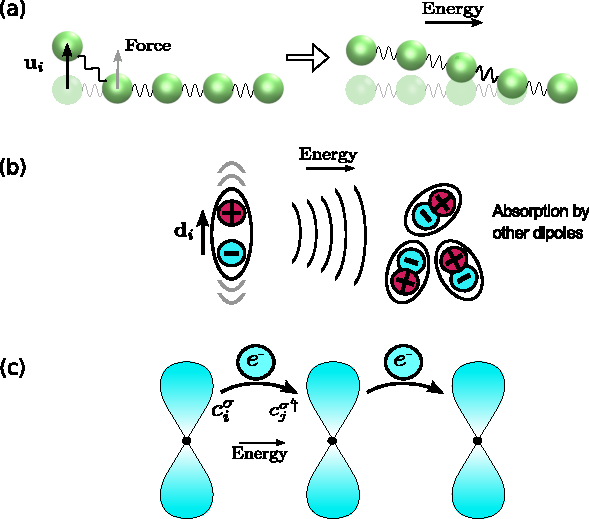
\includegraphics[width=.99\columnwidth]{inkscape/mechanisms.pdf}
 \caption{Schematic illustration of microscopic energy transfer mechanisms: (a) vibrational, (b) electromagnetic, and (c) electronic energy transfer. In phononic transfer, an atom displaced from its equilibrium position exerts a force on the neighboring atoms, giving rise to the propagation of displacement and transfer of energy. Fluctuations in the dipole moment, on the other hand, produce electromagnetic fields carrying energy, which can be absorbed by other dipoles. Electronic energy transfer arises from the hopping of electrons between atomic orbitals, driven by imbalance in electron number or temperature. Electron hopping is mathematically described here by the electron creation and annihilation operators.}
 \label{fig:mechanisms}
\end{figure}

Different energy transfer mechanisms and their corresponding degrees of freedom are schematically illustrated in Fig. \ref{fig:mechanisms}. Vibrational heat transfer in solids arises from the displacements $u_i^{\alpha}$ of each atom $i$ from their equilibrium positions to co-ordinate directions $\alpha\in\{x,y,z\}$. An atom displaced from its equilibrium position exerts a net force on other atoms, thereby leading to the propagation of displacement and transfer of energy. Similarly, electromagnetic energy is generated by fluctuations in local dipole moments $p_i^{\alpha}=qd_i^{\alpha}$, where $q$ is the dipole charge and $d_i^{\alpha}$ the dipole displacement in direction $\alpha$ \cite{rosa10}. The radiated electromagnetic energy propagates according to the Maxwell equations \cite{novotny}, scattered and absorbed by other dipoles. 

Quantum-mechanical electron transport in solids can be intuitively described by the tight-binding model \cite{ashcroftmermin}, in which electrons move by ''hopping'' between electron orbitals localized at individual atoms. Mathematically, the dynamics of a single electron is governed by the one-particle Schr\"odinger equation \cite{griffiths_qm}, but to capture fluctuations and dissipation, it is more practical to formulate the dynamical equations for electron creation and annihilation operators $c_i^{\sigma\dagger}$ and $c_i^{\sigma}$ \cite{ballentine}, which create and annihilate electrons at an orbital $\sigma$ localized at atom $i$, respectively\footnote{Label $\sigma$ is a composite index containing both the orbital wave function and electron spin.}. For notational simplicity, the same lattice subindex $i$ is used for each carrier to label the different spatial degrees of freedom. 

Modeling of energy transfer requires coupling at least some of the degrees of freedom to external reservoirs acting as sources and sinks for energy. With the exception of \citepub{twinning}, where Nos\'e-Hoover thermostats \cite{nose84,hoover85} are used, we employ Langevin baths as reservoirs in all works included in this thesis. The coupling of an atomic chain to Langevin baths is illustrated by a one-dimensional example in Fig. \ref{fig:langevin_chain}. In this case, the baths serve two purposes: The baths colored in red and blue act as external heat sources and sinks, respectively, and are used to drive energy through the system. The baths colored in green, on the other hand, mimic internal fluctuations and dissipation arising from anharmonic scattering, allowing for capturing non-linear effects in terms of effective relaxation rates \cite{bolsterli70}. This allows for a quantum-mechanical treatment of much larger systems than the more rigorous but computationally heavy Keldysh GF method \cite{haugjauho}, as discussed in more detail in \citepub{gf}. 

\begin{figure}
 \begin{center}
 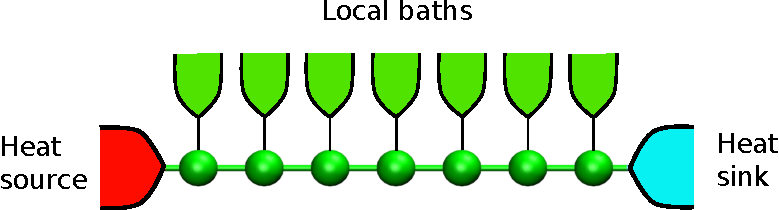
\includegraphics[width=.99\columnwidth]{inkscape/chain_baths.pdf}
 \caption{Schematic illustration of a chain of atoms coupled to Langevin baths. The baths at the left and right boundaries (red and blue) are at different temperatures and act as a heat source and sink, respectively. The baths colored in green describe internal fluctuations and dissipation arising from, e.g., phonon-phonon scattering.}
 \label{fig:langevin_chain}
  \end{center}
\end{figure}

\subsection{Equations of motion: common features}
\label{sec:th_eom}

The equations of motion for the three degrees of freedom $\bu_i$, $\bb{d}_i$, and $c_i^{\sigma}$ are all connected through the Langevin physics describing fluctuations and dissipation, leading to a similar solution method and phenomenology despite involving different energy carriers. The equations read  \cite{bolsterli70,rosa10,rosa11,dhar03}
\begin{subequations}
\begin{align}
 m_i \ddot{\bu}_i(t) &=  - \sum_j \bb{K}_{ij}\bb{u}_j(t) + \xi_i(t) - m_i \gamma \dot{\bu}_i, \label{eq:th_eom1} \\
 m_i \ddot{\bb{d}}_i(t) &= - \sum_j \bb{K}_{ij} \bb{d}_j(t) +q\sum_{j} \bb{E}_{ij}(t)+\xi_i(t)+ q\Eenv(\br_i,t) - m_i \gamma \dot{\bd}_i(t), \label{eq:th_eom2}\\
 i\hbar \dot{c}_i^{\sigma}(t) &= -\sum_{j,\sigma'} t_{ij}^{\sigma\sigma'} c_j^{\sigma'}(t) +\eta_i^{\sigma}(t) - i\hbar \gamma_e c_i^{\sigma}(t) \label{eq:th_eom3}.
\end{align}
\end{subequations}
Here $\bu_i=[u_i^{x},u_i^y,u_i^z]^T$ and $\bd_i=[d_i^x,d_i^y,d_i^z]^T$ are written as three-dimensional vectors. Equations \eqref{eq:th_eom1}, \eqref{eq:th_eom2} and \eqref{eq:th_eom3} contain, generally speaking, four different kinds of parameters: inertial mass $m_i$ of atom or dipole $i$, coupling coefficients $\bb{K}_{ij}$, $\bE_{ij}$ and $t_{ij}^{\sigma\sigma'}$ coupling different degrees of freedom, Langevin noise terms $\xi_i$, $\Eenv$, and $\eta_i$ responsible for thermal fluctuations, and damping coefficients $\gamma$ and $\gamma_e$ accompanying the fluctuations according to the FDT (Sec. \ref{sec:th_langevin}). Noise terms $\xi_i$, $\Eenv$, and $\eta_i$ essentially describe thermal fluctuations in phonon, photon or electron number and are governed either by Bose-Einstein or Fermi-Dirac statistics as detailed in Sec. \ref{sec:th_langevin}. %The stochastic background field $\Eenv(\br_i,t)$ appearing in the dipole equation of motion \eqref{eq:th_eom3} and arising from the thermal fluctuations of the environment ensures balance between electromagnetic absorption and emission in thermal equilibrium \cite{rosa10}.

Equations \eqref{eq:th_eom1}, \eqref{eq:th_eom2} and \eqref{eq:th_eom3} are derived in more detail in Sec. \ref{sec:th_eom2}, but they can be easily understood intuitively. As an example, Eq. \eqref{eq:th_eom1} declares that the acceleration of atom $i$ is proportional to the sum of (i) the forces exerted by other atoms $j$, proportional for each atom pair $i,j$ to the force constant matrix $\bb{K}_{ij}$ calculated from interatomic potential energy, (ii) stochastic Langevin force $\xi_i$ modeling local thermal fluctuations, and (iii) friction term $m_i \gamma \dot{\bu}_i$ responsible for energy dissipation at rate $\gamma$. To highlight the similarities between different carriers, we have used the linear approximation for the interparticle force in equation \eqref{eq:th_eom1}, allowing for the direct solution of the equations of motion as shown in the following Subsection. This assumption is relaxed in Sec. \ref{sec:th_eom2} to allow for more exact treatment of non-linear forces, which are responsible for microscopic phonon-phonon interactions and therefore necessary in the calculation of, e.g., frequency-dependent mean free paths (\citepub{cnt}) and the thermal conductivity of twinning nanowires (\citepub{twinning}). 

It is worth noting that whereas equations \eqref{eq:th_eom1} and \eqref{eq:th_eom2} are purely real and involve second time-derivatives on the left-hand side, Eq. \eqref{eq:th_eom3} for the electron annihilation operator $c_i^{\sigma}$ is imaginary and involves only a single time-derivative. This difference is rooted in the fundamental property of quantum mechanics that time evolution is modeled by diffusion equation in imaginary time (Schr\"odinger equation), allowing for wave-like solutions in real time \cite{ballentine}.

\subsection{Solution of the Langevin equations in terms of Green's functions}
\label{sec:th_eom_solution}
The similarity of Eqs. \eqref{eq:th_eom1}, \eqref{eq:th_eom2}, and \eqref{eq:th_eom3} allows for solving the equations in a similar fashion. The differential equations are first turned into algebraic equations by Fourier transforming the equations\footnote{We define Fourier transformation $\tilde f(\omega)$ for any function $f(t)$ as
\begin{equation}
 \tilde f(\omega) = \int_{-\infty}^{\infty} dt e^{i\omega t} f(t) \label{eq:th_fourier}
\end{equation}
and the corresponding inverse transformation as
\begin{equation}
 f(t) = \int_{-\infty}^{\infty} \frac{d\omega}{2\pi} e^{-i\omega t}\tilde f(\omega). \label{eq:th_fourier_inv}
\end{equation}}.
With small rearrangement, one then gets three linear systems of equations:
\begin{subequations}
\begin{align}
   - & \sum_{j,\beta}  [m_i (\omega^2+i\gamma \omega) \delta_{ij}\delta_{\alpha\beta} - K_{ij}^{\alpha\beta}] \tilde{u}_j^{\beta}(\omega) = \tilde \xi_i^{\alpha}(\omega) \label{eq:th_eom_fourier_phonon} \\
  - &  \sum_{j,\beta} \left[m(\omega^2+i\gamma\omega) \delta_{ij}\delta_{\alpha\beta} - K_{ij}^{\alpha\beta} +q^2 \omega^2 \mu_0 \mathbb{G}^{\alpha\beta}(\br_i,\br_j;\omega) \right]\tilde{d}_j^{\beta}(\omega) \notag \\
  & \qquad = q\tilde{E}_{\textrm{env}}^{\alpha}(\br_i,\omega) + \tilde{\xi}^{\alpha}_i(\omega) \label{eq:th_eom_fourier_photon} \\ 
  &  \sum_{j,\sigma'} \left[\hbar (\omega+i\gamma_e) \delta_{ij}\delta_{\sigma\sigma'} + t_{ij}^{\sigma\sigma'} \right] \tilde c_j^{\sigma'}(\omega) = \tilde \eta_i^{\sigma}(\omega)  ,  \label{eq:th_eom_fourier_electron}
\end{align}
\end{subequations}
where the Fourier-transformed degrees of freedom and Langevin noise terms are marked by using a tilde as an overscore. Angular frequency is denoted by $\omega$, Kronecker symbol $\delta_{ij}$ is zero for $i\neq j$ and equal to unity for $i=j$, and the co-ordinate directions $\alpha,\beta \in \{x,y,z\}$ are written explicitly in Eqs. \eqref{eq:th_eom_fourier_phonon} and \eqref{eq:th_eom_fourier_photon}. In Eq. \eqref{eq:th_eom_fourier_photon}, the Fourier transform $\tilde{\bE}_{ij}(\omega)$ of the electric field $\bE_{ij}$ appearing in Eq. \eqref{eq:th_eom2} is written in terms of the the electromagnetic Green's dyadic $\mathbb{G}^{\alpha\beta}(\br_i,\br_j;\omega)$ as \cite{novotny}
\begin{equation}
 \tilde{E}_{ij}^{\alpha}(\omega) = q\omega^2 \mu_0 \sum_{\beta} \mathbb{G}^{\alpha\beta}(\br_i,\br_j;\omega)\tilde{d}_j^{\beta}(\omega), \label{eq:th_Eij}
\end{equation}
where $\mu_0$ is the vacuum permeability. The Green's dyadic $\mathbb{G}^{\alpha\beta}(\br_i,\br_j;\omega)$ is defined in Sec. \ref{sec:th_eom2_photon}. 

The linear systems of equations \eqref{eq:th_eom_fourier_phonon}, \eqref{eq:th_eom_fourier_photon} and \eqref{eq:th_eom_fourier_electron} can be written in matrix form by combining all degrees of freedom into single composite vectors by defining $\tilde{\bu}(\omega)=[\tilde u_1^x(\omega),\tilde u_1^y(\omega),\tilde u_1^z(\omega),\tilde u_2^x(\omega),\tilde u_2^y(\omega),\tilde u_2^z(\omega),\dots]^T$ and defining vectors $\tilde{\bd}(\omega)$ and $\tilde{\bb{c}}(\omega)$ similarly. The Langevin terms appearing on the right-hand sides of Eqs. \eqref{eq:th_eom_fourier_phonon}, \eqref{eq:th_eom_fourier_photon} and \eqref{eq:th_eom_fourier_electron} can be similarly written in vector form by accounting for the contribution of each bath $J$ on each degree of freedom. The bath label $J$ corresponds to either local baths, which contribute to the fluctuating force only at a single site, or the environment field $\tilde{E}_{\textrm{env}}^{\alpha}(\br,\omega)$. More details of the labeling are given, e.g., in \citepub{gf}.

Following such a procedure, each of the equations \eqref{eq:th_eom_fourier_phonon}, \eqref{eq:th_eom_fourier_photon}, and \eqref{eq:th_eom_fourier_electron} can be written in the matrix form
\begin{equation}
 \bb{A}(\omega) \tilde{\bb{x}}(\omega) = \sum_J \tilde \zeta^J(\omega). \label{eq:th_general}
\end{equation}
where $\bb{A}(\omega)$ is a coefficient matrix multiplying the degrees of freedom $\tilde{\bb{x}}(\omega)$ (standing for $\tilde{\bu}(\omega)$, $\tilde{\bb{c}}(\omega)$, or $\tilde{\bb{d}}(\omega)$ written in vector form) in Eqs. \eqref{eq:th_eom_fourier_phonon}, \eqref{eq:th_eom_fourier_photon}, and \eqref{eq:th_eom_fourier_electron}. The coefficient matrix $\bb{A}(\omega)$ captures all physical details of the system's deterministic dynamics, including coupling between different degrees of freedom and dissipation arising from the baths. The right-hand side of Eq. \eqref{eq:th_general} is the sum over stochastic Langevin force contributions $\zeta^J$ (standing for $\xi$, $\eta$, or $\Eenv$) from each bath $J$ as discussed above.  

Equation \eqref{eq:th_general} can be solved by defining the GF as the matrix inverse $\bb{G}(\omega)=\bb{A}(\omega)^{-1}$ so that  
\begin{equation}
 \tilde{\bb{x}}(\omega)  =  \bb{G}(\omega) \sum_J \tilde \zeta^J(\omega). \label{eq:th_gf_solution}
\end{equation}
Equation \eqref{eq:th_gf_solution} can be straightforwardly interpreted: system's dynamics at each frequency is defined by the stochastic fluctuations from each bath at the same frequency, with the GF acting as the ''transfer matrix''. Our discrete formulation of the equations of motion allows for writing the GF as a matrix, but corresponding formulation for continuous medium would turn the GF into a function of two continuous variables $\br$, $\br'$. In this case, matrix sums in Eqs. \eqref{eq:th_general} and \eqref{eq:th_gf_solution} would be replaced by an integral.

The matrix GF $\bb{G}(\omega)$ is generally of the form \cite{datta}
\begin{equation}
 \bb{G}(\omega) = \left[\bb{G}^0(\omega)^{-1} - \sum_J \Sigma^J(\omega) \right]^{-1},
\end{equation}
where $\bb{G}^0(\omega)$ is the GF in absence of dissipation (i.e., Langevin baths) and bath self-energy matrices $\Sigma^J(\omega)$ describe the dissipation and energy level renormalization arising from the interaction with each bath $J$. For example, the self-energy corresponding to the bath at site $k$, introducing a friction term $m_i\gamma \dot{\bu}_k$ in the equation of motion for $\bu_k$, is $[\Sigma(\omega)]_{ij}=-im_i\gamma \omega \delta_{ij} \delta_{ik}\unitdyadic$. Here $\unitdyadic$ is the $3\times3$ unit matrix. 

With the FDT for the force variances $\langle \zeta^J(\omega) \zeta^J(\omega')^T \rangle$ presented in Sec. \ref{sec:th_langevin} and the solution \eqref{eq:th_gf_solution} available, one can calculate the thermal averages of any observable of interest. The calculation of heat current $ Q_i^{\textrm{bath}}$ to bath $i$, which represents the locally dissipated power, leads to a Landauer-B\"uttiker-like expression \cite{landauer57,buttiker92} as outlined in Sec. \ref{sec:th_currents} and shown in detail in \citepub{gf}. 

\section{Equations of motion: Carrier-specific details}
\label{sec:th_eom2}

\subsection{Phonons}

\label{sec:th_eom2_phonon}

We now move on to carrier-specific details leading to the linear Langevin equations \eqref{eq:th_eom1}, \eqref{eq:th_eom2}, and \eqref{eq:th_eom3}, starting from phonon heat transfer. The general equations of motion governing lattice dynamics are dictated by the lattice Hamiltonian \cite{ziman}
\begin{equation}
 \ca{H}_{\textrm{ph}} = \sum_{i=1}^N \frac{(\bp^{\textrm{kin}}_i)^2}{2m_i} + \ca{V}(\bb{r}_1,\dots,\bb{r}_N). \label{eq:th_hamiltonian}
\end{equation}
Here $\br_i$, $\bp^{\textrm{kin}}_i$, and $m_i$ are the position, kinetic momentum and mass of atom $i$, respectively. The total number of atoms (which can also be infinite) is denoted by $N$. The first term of Eq. \eqref{eq:th_hamiltonian} is the total kinetic energy of the atoms and the second term $\ca{V}$ is the interatomic potential energy responsible for the interatomic interactions. The choice of the potential energy function $\ca{V}$ is crucial for an accurate description of the lattice dynamics and, consequently, of energy transfer. In this thesis, we employed the Lennard-Jones \cite{allentildesley}, Tersoff \cite{tersoff88a}, Stillinger-Weber \cite{stillinger85}, and Fermi-Pasta-Ulam \cite{fermi55} potentials for modeling interatomic interactions in different systems.  

Applying Hamilton's equations of motion $\dot{\br}_i=\partial \ca{H}_{\textrm{ph}}/\partial \bp_i^{\textrm{kin}}$ and $\dot{\bp}_i^{\textrm{kin}}=-\partial \ca{H}_{\textrm{ph}}/\partial \br_i$ \cite{fetter} accompanied by stochastic Langevin terms \cite{dhar06} gives the equations of motion
\begin{equation}
 m_i \ddot{\br}_i(t) = \bb{F}_i(t) + \xi_i(t) - m_i \gamma \dot{\bb{r}}_i(t), \label{eq:th_eom}
\end{equation}
where the deterministic force acting on atom $i$ is
\begin{equation}
 \bb{F}_i = - \frac{\partial \ca{V}}{\partial \bb{r}_i}. \label{eq:th_force}
\end{equation}
As discussed in Sec. \ref{sec:th_eom}, the Langevin terms $\xi_i$ and $m_i\gamma \dot{\bb{r}}_i$ generally have two roles in the modeling of heat transfer. They are used both for (i) coupling atoms located at system's boundaries to external heat sources and sinks,  and (ii) to describe dissipative processes, if non-linear interactions accounting for phonon-phonon interactions are neglected. The form of the friction term $m_i \gamma \dot{\bb{r}}_i(t)$, proportional only to instantaneous velocity, is called Ohmic due to its analogue with a resistor in an electrical circuit \cite{weiss}. In general, the friction term is a time convolution giving rise to frequency-dependent damping \cite{weiss}, but in all publications included in this thesis, only the Ohmic form is used due to its simplicity.
 
Equation \eqref{eq:th_eom} generally describes the motions of atoms and molecules in solid, gas, and liquid systems. In solids, the atoms vibrate close to their equilibrium positions $\br_i^0$ and one can gain more insight into the lattice dynamics by focusing on the regime with small displacements from the equilibrium. The equilibrium positions $\br_i^0$ are defined by the condition of zero force on each atom:
\begin{equation}
 \left. \frac{\partial \ca{V}}{\partial \br_i} \right|_{\br_j=\br_j^0 \forall j} = 0. \label{eq:th_zeroforce}
\end{equation}
Assuming that the atoms remain close to the equilibrium positions, one can expand the potential energy in Taylor series in terms of the displacements $\bu_i=\br_i-\br_i^0$ \cite{ziman}:
\begin{equation}
 \ca{V} = \ca{V}_0 + \frac{1}{2} \sum_{i,j} \sum_{\alpha,\beta} u_i^{\alpha} K_{ij}^{\alpha \beta} u_j^{\beta}  + \frac{1}{6} \sum_{i,j,k} \sum_{\alpha,\beta,\gamma} \Upsilon_{ijk}^{\alpha\beta\gamma}  u_i^{\alpha} u_j^{\beta} u_k^{\gamma} + \mathcal{O}(u^4). \label{eq:th_V_taylor} % B_{ijk}^{\alpha\beta\gamma}
\end{equation}
In contrast to Eq. \eqref{eq:th_eom}, the Cartesian coordinate directions $\alpha,\beta \in \{x,y,z\}$ have been written here explicitly. The constant term $\ca{V}_0$ in Eq. \eqref{eq:th_V_taylor} does not play a role in dynamics, the first-order derivative term is zero due to Eq. \eqref{eq:th_zeroforce}, and the second-order term is proportional to the harmonic force constant (or ''spring'' constant) \cite{ziman}
\begin{equation}
 K_{ij}^{\alpha\beta} = \left. \frac{\partial^2 \ca{V}}{\partial u_i^{\alpha} \partial u_j^{\beta}} \right|_{\bu=\mathbf{0}}. \label{eq:th_K_def}
\end{equation}
The third term on the right-hand side of Eq. \eqref{eq:th_V_taylor} is proportional to the first-order anharmonic force constants
\begin{equation}
 \Upsilon_{ijk}^{\alpha\beta\gamma} = \left. \frac{\partial^3 \ca{V}}{\partial u_i^{\alpha} \partial u_j^{\beta} \partial u_k^{\gamma}} \right|_{\bu=\mathbf{0}}.
\end{equation}
The first and higher-order anharmonic terms correspond to phonon-phonon interactions \cite{ziman} responsible for anharmonic scattering. First-principles calculation of thermal conductivities and phonon mean free paths requires explicitly including these terms in the equations of motion. The non-linearity of the resulting equations prevents, however, their direct solution, so one needs to turn either to computationally heavy Keldysh GF techniques \cite{wang08} or simulating lattice dynamics using the classical MD method \cite{allentildesley}. MD is used in Publications \cp{spectral}, \cp{cnt}, \cp{twinning}, \cp{fpu}, and \cp{fpu2} due to its flexibility and applicability to large system sizes. MD is reviewed in Sec. \ref{sec:methods_md}.

At sufficiently low temperatures or when dissipative events can be modeled in terms of a given relaxation time, anharmonic terms can be neglected. Including only the two first terms in the right-hand side of Eq. \eqref{eq:th_V_taylor} in the equation of motion \eqref{eq:th_eom} for the atomic displacement $\bu_i=\br_i-\br_i^0$ gives the system of linear equations \eqref{eq:th_eom1}, repeated here for convenience:
\begin{equation}
 m_i \ddot{\bu}_i(t) =  - \sum_j \bb{K}_{ij}\bb{u}_j(t) + \xi_i(t) - m_i \gamma \dot{\bu}_i.  \tag{\ref{eq:th_eom1}}
\end{equation}
The linearity of Eq. \eqref{eq:th_eom1} allows for direct solution in frequency domain as discussed in Sec. \ref{sec:th_eom_solution} and, consequently, including quantum statistics through the quantum FDT for the noise terms $\xi_i$ (Sec. \ref{sec:th_langevin}). \change{By Fourier-transforming Eq.} \eqref{eq:th_eom1} \change{and re-organizing, one obtains the solution}
 \begin{equation}
 \tilde {\bu}_i(\omega) =  \sum_j \bb{G}_{ij}(\omega) \tilde{\xi}_j(\omega) , \label{eq:th_gf_phonon}
\end{equation}
\change{where the phonon Green's function is the inverse $\bb{G}(\omega)=\bb{A}^{\textrm{ph}}(\omega)^{-1}$ of the matrix $\bb{A}^{\textrm{ph}}(\omega)$ with $3\times 3$ block elements}
\begin{equation}
 \bb{A}_{ij}^{\textrm{ph}}(\omega)= -m_i(\omega^2+i\gamma\omega) \unitdyadic \delta_{ij} + \bb{K}_{ij} .
\end{equation}
\change{Solution }\eqref{eq:th_gf_phonon} \change{is used in Sec. \ref{sec:th_bathcurrents} to derive an expression for the local heat current flowing to each bath.}


\subsection{Photons}
\label{sec:th_eom2_photon}
Energy transfer by electromagnetic waves is described by the Maxwell equations \cite{jackson}. In the non-magnetic materials with no free charges as considered in this work, the electromagnetic fields arise from the fluctuating electric polarization fields inside the bodies, and the Maxwell equations for the electric field $\bE(\br,t)$ and magnetic field $\bb{H}(\br,t)$ read \cite{novotny}
\begin{subequations}
\begin{align}
  \nabla \times \bE(\br,t) + \mu_0 \frac{\partial \bb{H}(\br,t)}{\partial t} &= 0 , \label{eq:th_maxwell1} \\
  \nabla \times \bb{H}(\br,t) - \varepsilon_0 \frac{\partial \bb{E}(\br,t)}{\partial t} &=  \bb{j}(\br,t) , \label{eq:th_maxwell2} \\
   \nabla \cdot \bb{H}(\br,t) &= 0, \\
   \varepsilon_0 \nabla \cdot  \bb{E}(\br,t) &= -\nabla \cdot \bb{P}(\br,t).
\end{align}
\end{subequations}
Here, $\mu_0$ and $\varepsilon_0$ are the magnetic permeability and permittivity of vacuum, respectively. The polarization current $\bb{j}(\br,t)=\partial \bb{P}(\br,t)/\partial t$ defined in terms of the polarization density $\bb{P}(\br,t)$ appears as a source term in Eq. \eqref{eq:th_maxwell2}, giving rise to an electromagnetic field according to Eqs. \eqref{eq:th_maxwell1} and \eqref{eq:th_maxwell2}. The radiated electromagnetic field carries an energy flux, whose magnitude and direction are given by the Poynting vector $\bb{S}(\br,t)=\bb{E}(\br,t)\times \bb{H}(\br,t)$ \cite{novotny}. The polarization density consists of stochastic and electrically induced contributions \cite{benabdallah11} as discussed below. 

To derive an equation of motion for the electric field alone, we calculate the curl of Eq. \eqref{eq:th_maxwell1}:
\begin{alignat}{2}
  \nabla \times \nabla \times \bE(\br,t) &= - \mu_0 \frac{\partial}{\partial t} \left[\nabla \times \bb{H}(\br,t) \right] .
\end{alignat}
By using Eq. \eqref{eq:th_maxwell2}, we get the Helmholtz equation for the electric field \cite{novotny}:
\begin{equation}
   \nabla \times \nabla \times \bE(\br,t) + \mu_0 \varepsilon_0 \frac{\partial ^2\bb{E}(\br,t)}{\partial t^2}=  - \mu_0 \frac{\partial^2 \bb{P}(\br,t)}{\partial t^2}. \label{eq:th_eom_photons} % \label{eq:th_curlcurlE}
\end{equation}

To separate the fluctuating terms in the polarization density $\bb{P}(\br,t)$ in Eq. \eqref{eq:th_eom_photons}, we divide the polarization density into the induced and fluctuating parts as $\bb{P}(\br,t)=\bb{P}_{\textrm{ind}}(\br,t)+ \bb{P}_{\textrm{fluc}}(\br,t)$ \cite{benabdallah11}. In the linear and local approximation, the induced part is proportional to the electric field in the frequency domain \cite{novotny}:
\begin{equation}
 \tilde{\bb{P}}_{\textrm{ind}}(\br,\omega)= \varepsilon_0 \chi(\br,\omega) \tilde{\bb{E}}(\br,\omega), \label{eq:th_P_chi}
\end{equation}
where $\chi(\br,\omega)$ is the susceptibility. The imaginary part of $\chi(\br,\omega)$ is responsible for dielectric losses \cite{jackson}. The fluctuating polarization density $\bb{P}_{\textrm{fluc}}(\br,t)$ is the analogue of the Langevin force and its variance in frequency-domain is proportional to the imaginary part of $\chi(\br,\omega)$ through the FDT presented in Sec. \ref{sec:th_langevin}.

Equation \eqref{eq:th_P_chi} lumps the complex response of the medium to the local electric field into a single, macroscopic parameter $\chi(\br,\omega)$. While such a macroscopic description has been used with great success to model energy transfer by electromagnetic fields in the framework of fluctuational electrodynamics \cite{rytov} (see, e.g., Refs. \cite{volokitin07} and \cite{joulain05} for reviews), it is expected to break down in nanoscale \cite{chalopin12b}. 

A more microscopic model for fluctuating polarization fields was introduced by Rosa \textit{et al.} \cite{rosa10,rosa11} for the purpose of quantizing electromagnetic fields in lossy media. They modeled the polarization as a collection of dipoles $\bp_i$ located at points $\br_i$, corresponding to the dipole density
\begin{equation}
 \bb{P}(\br,t) = \sum_i \bp_i(t) \delta(\br-\br_i).
\end{equation}
The dynamics of each dipole was modeled by the classical oscillator model with mass $m_i$ and resonance angular frequency $\omega_0$ so that the Langevin equation of motion for the dipole displacement $\bd_i=\bp_i/q$ reproduces Eq. \eqref{eq:th_eom2} (with $K_{ij}^{\alpha\beta}=m\omega_0^2\delta_{ij}\delta_{\alpha\beta}$): \cite{rosa10,rosa11}
\begin{equation}
 m_i \ddot{\bb{d}}_i(t) = - m \omega_0^2 \bb{d}_i(t) +q\sum_{j} \bb{E}_{ij}(t)+\xi_i(t)+ q\Eenv(\br_i,t) - m_i \gamma \dot{\bd}_i(t). \label{eq:th_eom2b}
\end{equation}
The stochastic Langevin force $\xi_i$ and friction $m_i\gamma \dot{\bd}_i$ account for mechanical fluctuations and dissipation in dipole dynamics, respectively, and are equivalent to the corresponding Langevin terms in the phonon equation of motion \eqref{eq:th_eom}. The thermal background field $\Eenv(\br_i,t)$ acts as a similar noise term, corresponding to electromagnetic absorption of energy from the radiation field. To ensure balance between electromagnetic absorption and emission in thermal equilibrium, there must be an accompanying dissipative term in the equation of motion. Such a term is found in the local field $\bE_{ii}$, which manifests as Abraham-Lorentz radiation damping in the dipole motion \cite{jackson} as discussed in more detail in \citepub{dipole}. 

The local electric field $\bE_{ij}$ acting as a force term in Eq. \eqref{eq:th_eom2} and coupling different dipoles can be written in frequency-domain as [Eq. \eqref{eq:th_Eij}] \cite{novotny,rosa11}:
\begin{equation}
 %\tilde \bE(\br,\omega) = \tilde \bE_0(\br,\omega) + i \omega \mu_0 \int_V d\mathbf{r}' \mathbb{G}(\br,\br';\omega) \tilde{\bb{j}}(\br',\omega). \label{eq:th_Etilde}
\tilde \bE_{ij}(\omega) = \omega^2 \mu_0 \mathbb{G}(\br_i,\br_j;\omega) \tilde{\bb{p}}_j(\omega), \tag{\ref{eq:th_Eij}}
\end{equation}
where $\mathbb{G}(\br,\br';\omega)$ is the electromagnetic Green's dyadic found by solving Eq. \eqref{eq:th_eom_photons} in frequency-domain for a point-like dipole at $\br'$ \cite{novotny}:
 \begin{equation}
 \nabla \times \nabla \times \gem(\bb{r},\br';\omega) - (\omega^2/c^2) \epsenv(\br,\omega)\gem(\bb{r},\br';\omega)  =  \delta(\bb{r}-\br')\unitdyadic. \label{eq:intro_gemdef}
\end{equation}
For generality, we have assumed that the point-like dipole is located in an inhomogeneous environment with dielectric constant $\epsenv(\br,\omega)$ to allow for modeling dipole-dipole energy transfer in a mirror cavity as in \citepub{dipole}. The calculation of Green's dyadics for planar multilayer geometries has been presented by Toma\v{s} \cite{tomas95}. By Fourier transforming Eq. \eqref{eq:th_eom2}, substituting Eq. \eqref{eq:th_Eij} and rearranging one gets the linear system of equations corresponding to Eq. \eqref{eq:th_eom_fourier_photon} for the dipole displacements:
\begin{alignat}{2}
 - & \sum_{j,\beta} \left[m(\omega^2-\omega_0^2+i\gamma\omega) \delta_{ij}\delta_{\alpha\beta} +q^2 \omega^2 \mu_0 \mathbb{G}^{\alpha\beta}(\br_i,\br_j;\omega) \right]\tilde{d}_j^{\beta}(\omega) \notag \\
  & \qquad = q\tilde{E}_{\textrm{env}}^{\alpha}(\br_i,\omega) + \tilde{\xi}^{\alpha}_i(\omega). \label{eq:th_eom_fourier_photon_b}
\end{alignat}

While Eq. \eqref{eq:th_eom_fourier_photon_b} is very similar to the corresponding (linearized) equation \eqref{eq:th_eom_fourier_phonon} for phonon heat transfer, there are some differences. In contrast to the static interatomic force constants $K_{ij}^{\alpha\beta}$ appearing in the phonon equation of motion, the dipole-dipole coupling coefficients $\mathbb{G}^{\alpha\beta}(\br_i,\br_j;\omega)$ are (i) frequency-dependent and (ii) depend on the electromagnetic environment through the dielectric constant $\epsenv(\br,\omega)$. The dipole-dipole coupling coefficients $\mathbb{G}^{\alpha\beta}(\br_i,\br_j;\omega)$ can also be very long-ranged, allowing for energy transfer across large distances even in vacuum. These differences between phononic and photonic energy transfer are, however, related to our somewhat artificial separation between lattice vibrations and electromagnetic field. A fully coupled model of lattice vibrations and electromagnetic field \cite{chiloyan15} enables, e.g., tunneling of acoustic phonon energy across vacuum \cite{prunnila10}.

\subsection{Electrons}
\label{sec:th_eom2_electron}

First-principles modeling of electron transport starts from the quantum-mechanical Hamiltonian $\ca{H}_{\textrm{el}}$ for electrons and ions constituting the atomic lattice \cite{ashcroftmermin}. For the simplicity of discussion, we exclude electron-electron, electron-phonon, and electron-photon interactions so that the single-particle Hamiltonian for an electron moving in the (static) potential generated by the ions located at points $\bb{R}_i$ is \cite{ashcroftmermin}
\begin{equation}
 \ca{H}_{\textrm{el}} = - \frac{\hbar^2}{2m_e} \nabla^2  + \sum_i V(\br-\bb{R}_i), \label{eq:th_Hel}
\end{equation}
where $m_e$ is the electron mass and $V(\br-\bb{R}_i)$ is the electrostatic potential from ion $i$. To arrive at the tight-binding approximation, we first solve the eigenstates $\phi_i^{\sigma}$ and the corresponding eigenenergies $E_i^{\sigma}$ for a \textit{single} ion:
\begin{equation}
 \left[ - \frac{\hbar^2}{2m_e} \nabla^2  +  V(\br-\bb{R}_i) \right] \phi_i^{\sigma} (\br) = E_i^{\sigma} \phi_i^{\sigma}(\br). \label{eq:th_schrode}
\end{equation}
Here the eigenstates are labeled by the superscript $\sigma$. The localized solutions of Eq. \eqref{eq:th_schrode} are centered around $\bb{R}_i$ due to the attractive ion potential $V(\br-\bb{R}_i)$. The tight-binding approximation is to assume that the localized orbitals $\phi_i^{\sigma}$ for each atom $i$ form a complete set \footnote{Typically only a small subset is used, as tightly bound states do not need to be included. More generally, Wannier functions can be used as basis functions \cite{ashcroftmermin}.} so that the electron eigenstates of Hamiltonian \eqref{eq:th_Hel} can be written as
\begin{equation}
 \psi(\br) = \sum_{i,\sigma} b_i^{\sigma} \phi_{i}^{\sigma}(\br).
\end{equation}
The Hamiltonian matrix elements of the basis functions are
\begin{alignat}{2}
 \langle \phi_i^{\sigma} | \ca{H}_{\textrm{el}} | \phi_j^{\sigma'} \rangle &= \left\langle \phi_i^{\sigma} \left| - \frac{\hbar^2}{2m_e} \nabla^2  +V(\br-\bb{R}_i)+ \sum_{k\neq i} V(\br-\bb{R}_k) \right |\phi_j^{\sigma'} \right\rangle \\
 &= E_i^{\sigma} \langle \phi_i^{\sigma}|\phi_j^{\sigma'} \rangle + \left\langle \phi_i^{\sigma} \left| \sum_{k\neq i} V(\br-\bb{R}_k) \right| \phi_j^{\sigma'} \right\rangle \label{eq:th_Helements1} \\
  & = E_i^{\sigma} \langle \phi_i^{\sigma}|\phi_j^{\sigma'} \rangle  - \tilde t_{ij}^{\sigma\sigma'}, \label{eq:th_Helements}
\end{alignat}
where we used Eq. \eqref{eq:th_schrode} in Eq. \eqref{eq:th_Helements1} and also defined the ''hopping'' matrix element as 
\begin{equation}
  \tilde t_{ij}^{\sigma\sigma'} = - \int d\bb{r} \phi_i^{\sigma}(\br)^*  \sum_{k\neq i} V(\br-\bb{R}_k)   \phi_j^{\sigma'}(\br).
\end{equation}
Assuming for simplicity that the overlap matrix element $\langle \phi_i^{\sigma}| \phi_j^{\sigma'} \rangle$ is small for $i\neq j$ so that the orbitals form an orthogonal basis, one can write the tight-binding Hamiltonian corresponding to the matrix elements of Eq. \eqref{eq:th_Helements} in the braket notation \cite{schwabl} as 
\begin{equation}
 \ca{H}_{\textrm{el}}^{\textrm{tb}} = \sum_{i,j} \sum_{\sigma,\sigma'} (E_i^{\sigma} \delta_{ij}\delta_{\sigma\sigma'}  - \tilde t_{ij}^{\sigma\sigma'})|\phi_i^{\sigma} \rangle \langle \phi_j^{\sigma'} | . \label{eq:th_Hel_tb}
\end{equation}
The equivalent second-quantized form \cite{schwabl} for the Hamiltonian \eqref{eq:th_Hel_tb} is
\begin{equation}
 \ca{H}_{\textrm{el}}^{\textrm{tb}} = \sum_{i,j} \sum_{\sigma,\sigma'} (E_i^{\sigma} \delta_{ij}\delta_{\sigma\sigma'}  - \tilde t_{ij}^{\sigma\sigma'}) c_i^{\sigma\dagger} c_j^{\sigma'}, \label{eq:th_Hel_tb_final}
\end{equation}
where the electron creation operator $c_i^{\sigma\dagger}$ creates electrons at orbital $\phi_i^{\sigma}$ and annihilation operator $c_j^{\sigma'}$ annihilates electrons at orbital $\phi_j^{\sigma'}$:
 \begin{subequations}
  \begin{align} 
     c_i^{\sigma\dagger} |0 \rangle = | \phi_i^{\sigma} \rangle,  \\
     c_j^{\sigma'} |\phi_j^{\sigma'} \rangle = | 0 \rangle.
  \end{align}
 \end{subequations}
Here $|0\rangle$ is the vacuum state with no electrons. 

With the Hamiltonian of Eq. \eqref{eq:th_Hel_tb_final}, the Heisenberg equation of motion $i\hbar \dot{c}_i^{\sigma} = - \left[\ca{H}_{\textrm{el}}^{\textrm{tb}},c_i^{\sigma} \right]$ \cite{ballentine} accompanied by the stochastic Langevin force $\eta_i^{\sigma}$ and Ohmic damping $-i\hbar \gamma_e c_i^{\sigma}(t)$ \cite{dhar03} leads to the equation of motion \eqref{eq:th_eom3}:
\begin{equation}
 i\hbar \dot{c}_i^{\sigma}(t) = -\sum_{j,\sigma'} t_{ij}^{\sigma\sigma'} c_j^{\sigma'}(t) +\eta_i^{\sigma}(t) - i\hbar \gamma_e c_i^{\sigma}(t) \tag{\ref{eq:th_eom3}}.
\end{equation}
Here the orbital energy $E_i^{\sigma}$ was absorbed to the hopping constant through the definition 
\begin{equation}
 t_{ij}^{\sigma\sigma'}=\tilde t_{ij}^{\sigma\sigma'}-E_{i}^{\sigma}\delta_{ij}\delta_{\sigma\sigma'}.
\end{equation}

The Langevin terms $\eta_i^{\sigma}$ and $-i\hbar \gamma_e c_i^{\sigma}$ in Eq. \eqref{eq:th_eom3} are responsible for fluctuations in electron number and thereby act essentially as additional scattering channels. This idea of modeling inelastic effects by additional scattering channels is due to B\"uttiker \cite{buttiker86} and d'Amato and Pastawski \cite{damato90}, and it greatly simplifies the modeling of dephasing and dissipation events in quantum transport compared to the more rigorous but computationally demanding perturbative Keldysh GF techniques \cite{haugjauho}.

Equation \eqref{eq:th_eom3} is formally similar to the phonon equation of motion \eqref{eq:th_eom1}, with the hopping constants $t_{ij}^{\sigma\sigma'}$ playing the role of force constants $K_{ij}^{\alpha\beta}$. Differences arise from, e.g., the first-order time derivative in the equation for electrons. As a consequence, there is no simple correspondence between the electron dynamics at energies $E$ and $-E$ [described by the terms $c_i^{\sigma}(E/\hbar)$ and $c_i^{\sigma}(-E/\hbar)$] whereas for phonons, one can restrict the analysis to positive frequencies due to the identity $\tilde{\bu}_i(\omega)^*=\tilde{\bu}_i(-\omega)$. As a second difference, electron occupation at thermal equilibrium obeys Fermi-Dirac statistics with chemical potential $\mu$ and temperature $T$, which is evident in the FDT discussed in Sec. \ref{sec:th_langevin}. As is well-known from solid-state physics \cite{ashcroftmermin}, only electrons with energies close to the chemical potential $\mu$ participate in transport, allowing for the relatively easy control of electron flow by the tuning of $\mu$ by an external electrostatic potential. For phonons, such a tuning mechanism does not generally exist. One can, however, envision using phononic crystals \cite{maldovan13} for the transmission and blocking of specific frequencies, potentially allowing for similar control of the phonon transport band as for electrons.  

% For phonons, the statistics at thermal equilibrium is Bose-Einstein distribution with the chemical potential $\mu=0$. As a consequence, thermal transport by phonons is always broadband with a large range of frequencies \footnote{Except at very low temperatures, where only a narrow range of phonons close to the zero-frequency can be excited.} \cite{ziman}. 


\section{Langevin theory}
\label{sec:th_langevin}

As noted earlier, Langevin theory is used throughout this thesis to model thermal fluctuations. In Langevin theory, the system under study is imagined to interact with an infinite collection of harmonic oscillators. With a few simplifying assumptions \cite{weiss}, one can integrate out the bath degrees of freedom so that their interactions with the system are effectively described by fluctuating and dissipative forces \cite{weiss,dhar06}. The fluctuating force is a random variable with zero average and its variance is fixed by the FDT \cite{nyquist28,callen51}, which relates the strength of fluctuations to the dissipation. FDT essentially ensures the onset of statistical thermal equilibrium when all bath temperatures are equal.

For Ohmic coupling to a bath of harmonic oscillators, assumed for atomic displacements in Eqs. \eqref{eq:th_eom1} and dipole displacements in Eq. \eqref{eq:th_eom2}, the variance of the Langevin force $\tilde{\xi}_i$ in frequency domain is related to the friction parameter $\gamma$ and bath temperature $T_i$ through the FDT \cite{weiss,dhar06}
\begin{equation}
 \langle \tilde \xi_i(\omega) \tilde \xi_i(\omega')^T \rangle = 4\pi \delta(\omega+\omega') \hbar \omega m_i \gamma \left[f_{\textrm{BE}}(\omega,T_i)+ \frac{1}{2} \right] \bb{I}_{3\times 3}. \label{eq:th_xixiom_ohmic_qm}
\end{equation}
Here the angular brackets stand for statistical ensemble average, the Bose-Einstein function is defined as
\begin{equation}
 f_{\textrm{BE}}(\omega,T)=\left[\exp(\hbar \omega/k_BT)-1\right]^{-1}, \label{eq:th_fBE}
\end{equation}
and the unit matrix $\unitdyadic$ reflects the independence of fluctuations in different coordinate directions. For the Ohmic coupling of electrons to a bath, the variance of the ''force'' $\tilde{\eta}_i$ appearing as a source term in Eq. \eqref{eq:th_eom3} is \cite{dhar03,dhar06b,roy07}
\begin{equation}
 \langle \tilde \eta_{i}^{\sigma\dagger}(\omega) \tilde \eta_{j}^{\sigma}(\omega') \rangle = 4\pi\delta(\omega-\omega') \gamma_e f_{\textrm{FD}}(\omega;\mu_{i},T_{i}) \delta_{ij}\delta_{\sigma\sigma'}, \label{eq:th_etaetaom}
\end{equation}
where $\mu_i$ is the bath chemical potential and 
\begin{equation}
 f_{\textrm{FD}}(\omega;T,\mu)=\left\{\exp\left[(\hbar \omega-\mu)/k_BT\right]+1\right\}^{-1}
\end{equation}
is the Fermi-Dirac function.

In the classical high-temperature limit ($k_B T \gg \hbar \omega$) relevant in the MD simulations of Publications \cp{spectral}, \cp{cnt}, \cp{fpu}, and \cp{fpu2}, FDT \eqref{eq:th_xixiom_ohmic_qm} reduces to the classical FDT
\begin{equation}
 \langle \tilde \xi_i(\omega) \tilde \xi_i(\omega')^T \rangle = 4\pi \delta(\omega+\omega') m_i \gamma k_B T_i  \bb{I}_{3\times 3}. \label{eq:th_xixiom_ohmic_classical}
\end{equation}
Equation \eqref{eq:th_xixiom_ohmic_classical} corresponds to memoryless friction, as evident from the same equation written in time-domain \cite{zwanzig}:
\begin{equation}
 \langle \xi_i(t)  \xi_i(t')^T \rangle = 2 m_i \gamma k_B T_i \delta(t-t') \bb{I}_{3\times 3}. \label{eq:th_xixit_ohmic_classical}
\end{equation}

For the thermal background field $\Eenvtilde(\br,\omega)$ arising from the environment with dielectric constant $\epsenv(\br,\omega)$ and temperature $\Tenv$, the FDT reads \cite{novotny}
\begin{equation}
 \langle \Eenvtilde(\br,\omega) \Eenvtilde(\br',\omega')^T \rangle = 4\pi \delta(\omega+\omega') \hbar \omega^2 \mu_0 \textrm{Im}[\mathbb{G}(\br,\br';\omega)] \left[f_{\textrm{BE}}(\omega,\Tenv)+ \frac{1}{2} \right], \label{eq:th_e0e0om}
\end{equation}
where the electric Green's dyadic was defined by Eq. \eqref{eq:intro_gemdef}. 

For completeness, let us finally present the FDT for the fluctuating polarization density $\bb{P}_{\textrm{fluc}}$ appearing through the relation $\bb{P}=\bb{P}_{\textrm{ind}}+\bb{P}_{\textrm{fluc}}$ in Eq. \eqref{eq:th_eom_photons}, because it acts as the basis of fluctuational electrodynamics \cite{rytov,lifshitz56} often used for the modeling of electromagnetic energy transfer \cite{joulain05,volokitin07}. In the local and isotropic approximation, the FDT reads \cite{novotny}
\begin{alignat}{2}
 & \left\langle \tilde{\bb{P}}_{\textrm{fluc}}(\br,\omega) \tilde{\bb{P}}_{\textrm{fluc}}(\br',\omega')^T\right\rangle \notag \\
 &\qquad = 4\pi \delta(\omega+\omega') \hbar \varepsilon_0 \textrm{Im}\left[ \chi(\br,\omega)\right] \delta(\br-\br') \left[f_{\textrm{BE}}(\omega,T)+\frac{1}{2}\right]  \unitdyadic, \label{eq:th_PflucPfluc}
\end{alignat}
where $\chi(\br,\omega)$ is the local susceptibility. 

\section{Energy currents and spectral analysis}
\label{sec:th_currents}
% Mathematical expressions for energy currents are needed to extract energy transfer rates from the microscopic theory. Energy currents are calculated from variations in the local energy as discussed below in Sec. \ref{sec:th_energybalance}. When non-linearities accounting for dissipative processes are neglected or modeled in terms of relaxation parameters, an analytical Landauer-B\"uttiker-like expression for energy currents can be derived as outlined in Sec. \ref{sec:th_bathcurrents}. This expression directly decomposes energy currents into spectral contributions, giving an insightful picture of energy flow at each frequency. For non-linear systems, the energy currents must be calculated numerically and such a spectral decomposition of heat current has not been available. Derivation of such an expression for the spectral heat current, applicable to non-linear phonon transport, is one of the main results of this thesis and is discussed in detail in Sec. \ref{sec:th_spectral_curr}.

The flow of energy is \change{typically} induced by spatial variations in temperature\footnote{In the case of electrons, also spatial variations in chemical potential drive energy transfer.}. In the Langevin theory, temperature differences generate energy currents not only inside the system under study but also between the system and the heat baths. Heat currents to baths generally correspond either to energy transfer with the surroundings or the locally dissipated power, which both deliver important insight into the energy transfer in the system. In the linearized model of Sec. \ref{sec:th_eom1}, an analytical Landauer-B\"uttiker-like expression for the bath currents can be derived. This expression directly decomposes the energy current into its spectral contributions, giving an insightful picture of energy flow at each frequency.

For non-linear systems, energy currents in the system must be calculated from numerical simulations. So far, a spectral decomposition of heat current similar to the Landauer-B\"uttiker formula has, however, been unavailable for non-linear systems, complicating the identification of energy transfer mechanisms in systems with strong carrier-carrier scattering. Derivation of such a decomposition, applicable to phononic heat transfer in non-linear systems, is one of the main results of this thesis.

Energy currents are calculated from variations in the local energy as discussed below in Sec. \ref{sec:th_energybalance}. The derivation of the analytical Landauer-B\"uttiker-like expression for bath currents in linear systems is outlined in Sec. \ref{sec:th_bathcurrents}. The general spectral decomposition of heat current, applicable to non-linear phonon transport, is discussed in detail in Sec. \ref{sec:th_spectral_curr}. For the brevity of discussion, we focus below on energy transfer by phonons and only comment on the (small) differences to photonic and electronic energy transfer when relevant. 

% Energy currents are calculated from microscopic theory by monitoring variations in the local energy. 



\subsection{Local energy balance}
\label{sec:th_energybalance}
Expressions for energy currents can generally be inferred from the rate of change in local energy \cite{hardy63}. In lattice heat transfer, vibrational energy $e_i$ of each atom $i$ consists of the kinetic and potential energy contributions:
\begin{equation}
 e_i = \frac{1}{2}m_i\dot{\bu}_i^2 + \frac{1}{2} \sum_{\alpha,\beta}\sum_j u_i^{\alpha} K_{ij}^{\alpha\beta} u_j^{\beta} . \label{eq:th_ei}
\end{equation}
Here the first term is the kinetic energy and the second potential energy term has been written in the harmonic approximation \eqref{eq:th_V_taylor} for the simplicity of discussion. More general derivation of heat currents is given in Publication \cp{fpu}. Calculating the time derivative of Eq. \eqref{eq:th_ei}, using the Langevin equation of motion \eqref{eq:th_eom1}, and taking the ensemble average gives
\begin{equation}
 \left\langle \frac{de_i}{dt} \right\rangle =  -\sum_j  Q_{i\to j} -  Q_i^{\textrm{bath}} , \label{eq:th_ei_dot}
\end{equation}
where the term inside the sum is the heat current from atom $i$ to $j$,
\begin{equation}
 Q_{i \to j} = \frac{1}{2} \sum_{\alpha,\beta} \left\langle \dot{u}_i^{\alpha}K_{ij}^{\alpha\beta} u_j^{\beta} - u_i^{\alpha} K_{ij}^{\alpha\beta} \dot{u}_j^{\beta} \right\rangle. \label{eq:th_Qij}
\end{equation}
The second term on the right-hand side of Eq. \eqref{eq:th_ei_dot} is the current to the local heat bath:
\begin{equation}
 Q_i^{\textrm{bath}} = \langle [m_i\gamma \dot{\bu}_i-\xi_i] \cdot \dot{\bu}_i \rangle, \label{eq:th_Qibath}
\end{equation}
which is non-zero only for sites coupled to heat baths ($\gamma\neq 0$). The energy flow between neighboring atoms and to the baths in the Langevin bath model is depicted in Fig. \ref{fig:vib_currents}. 

The bath current term is present in Eq. \eqref{eq:th_ei_dot} for all atoms in the self-consistent heat bath model (\citepub{gf}), as all particles are coupled to heat baths mimicking scattering events driving the system to local thermal equilibrium. In the MD simulations of Publications \cp{spectral},\cp{cnt}, \cp{fpu}, and \cp{fpu2}, on the other hand, only atoms in the heat source and sink regions are coupled to heat baths, so the $Q_i^{\textrm{bath}}$ term is absent for most atoms. 

\begin{figure}
 \begin{center}
 \includegraphics[width=.59\columnwidth]{inkscape/bath_current.pdf}
 \end{center}
 \caption{Schematic illustration of vibrational heat flow to neighboring atoms and to the local bath.}
 \label{fig:vib_currents}
\end{figure}

Equation \eqref{eq:th_Qibath} is also valid for the locally dissipated power by dipoles, when the atomic displacement $\bb{u}_i$ is replaced by the dipole displacement $\bb{d}_i$. The derivation is based on calculating the rates of change in local electromagnetic and mechanical energy and is presented in \citepub{dipole}. One can similarly calculate microscopic expressions for electron currents from the rate of change in the local electron number \cite{roy07}. 

\subsection{Green's function calculation of bath currents}
\label{sec:th_bathcurrents}

To outline the calculation of the ensemble average of the bath heat current \eqref{eq:th_Qibath} in linearized phonon thermal conduction that can be analyzed analytically, we assume that the solution for the atomic displacements $\tilde{\bu}_i(\omega)$ at each site $i$ is given in terms of the GF matrix $\bb{G}(\omega)$ as [see Eq. \eqref{eq:th_gf_solution}]
\begin{equation}
 \tilde{\bu}_i(\omega) = \sum_{j} \bb{G}_{ij}(\omega) \tilde{\xi}_j(\omega).
\end{equation}
The thermal average of $Q_i^{\textrm{bath}}$ can then be calculated by substituting the Fourier transforms of $\bu_i$ and $\xi_i$ evaluated at time $t=0$ to Eq. \eqref{eq:th_Qibath} (thermal average of the current is time-independent). Noting that the Fourier transform of velocity $\dot{u}_i^{\alpha}(t)$ is given by $-i\omega \tilde{u}^{\alpha}_i(\omega)$, this procedure gives (\citepub{gf})
\begin{alignat}{2}
 Q_i^{\textrm{bath}}  &= \int_{-\infty}^{\infty} \frac{d\omega}{2\pi} \int_{-\infty}^{\infty} \frac{d\omega'}{2\pi} \sum_{\alpha} \langle  [ -im\gamma\omega \tilde u_i^{\alpha}(\omega)-\tilde \xi_i(\omega)][-i\omega' \tilde u_i^{\alpha}(\omega')] \rangle \\
  &= \int_{-\infty}^{\infty} \frac{d\omega}{2\pi} \int_{-\infty}^{\infty} \frac{d\omega'}{2\pi} \sum_{\alpha} \sum_{j,k} \sum_{\beta,\gamma} \left\langle \left[ -im\gamma\omega G_{ij}^{\alpha\beta}(\omega)\tilde \xi_j^{\beta}(\omega)-\tilde \xi_i^{\alpha}(\omega) \right] \right. \notag \\
  &\qquad \times \left.\left[-i\omega' G_{ik}^{\alpha\gamma}(\omega') \tilde \xi_k^{\gamma}(\omega') \right]  \right\rangle .
\end{alignat}
At this point, one can use the FDT \eqref{eq:th_xixiom_ohmic_qm} for correlations of the form $\langle \tilde \xi_j^{\beta}(\omega)\tilde \xi_k^{\gamma}(\omega') \rangle$, which eliminates one of the frequency integrals. Substituting the FDT, rearranging and using the definition of the local bath coupling function $[\Gamma^i(\omega)]_{jk}^{\alpha\beta}=2m_i\gamma\omega \delta_{\alpha\beta}\delta_{ij} \delta_{ik}$, one finally gets the multiprobe Landauer-B\"uttiker-like \cite{landauer57,buttiker92} expression (\citepub{gf})
\begin{equation}
  Q_i^{\textrm{bath}} = \int_0^{\infty} \frac{d\omega}{2\pi} \hbar \omega  \sum_j \ca{T}_{ij}(\omega) \left[ f_{\textrm{BE}}(\omega,T_j)- f_{\textrm{BE}}(\omega,T_i)\right]. \label{eq:th_QI}
\end{equation}
Here $T_i$ and $T_j$ are the temperatures of the baths at sites $i$ and $j$, and the transmission function between baths is defined as
\begin{equation}
 \ca{T}_{ij}(\omega) = \textrm{Tr}\left[\Gamma^i(\omega) \bb{G}(\omega) \Gamma^j(\omega) \bb{G}(\omega)^{\dagger} \right]. \label{eq:th_caroli}
\end{equation}
Equation \eqref{eq:th_caroli} is the well-known Caroli form for the transmission function \cite{caroli71}, originally derived for ballistic two-terminal electron transport and later for phonons \cite{mingo06,yamamoto06}. In the form written in Eq. \eqref{eq:th_caroli}, the expression for the transmission function remains valid also when the baths are non-Ohmic (see \citepub{gf}). 

In \citepub{dipole}, an expression similar to Eq. \eqref{eq:th_QI} was derived for the locally dissipated power by fluctuating dipole moments:
\begin{alignat}{2}
 Q_i^{\textrm{bath}} &= \int_0^{\infty}\frac{d\omega}{2\pi} \hbar\omega \sum_{j} \ca{T}_{ij}(\omega) \left[f_{\textrm{BE}}(\omega,T_j)-f_{\textrm{BE}}(\omega,T_i ) \right] \notag \\
  & \quad + \int_0^{\infty} \frac{d\omega}{2\pi} \hbar \omega \ca{T}_{i,\textrm{rad}}(\omega)\left[ f_{\textrm{BE}}(\omega,\Tenv)-f_{\textrm{BE}}(\omega,T_i)\right].
\end{alignat}
The dipole-dipole transmission function $\ca{T}_{ij}(\omega)$ and dipole-environment transmission $\ca{T}_{i,\textrm{rad}}(\omega)$ are given by expressions analogous to Eq. \eqref{eq:th_caroli}. The microscopic oscillator parameters $m$, $q$, $\omega_0$ and $\gamma$ appear, however, explicitly in these expressions through the GF $\bb{G}(\omega)$ and the bath coupling functions $\Gamma^i(\omega)$. When only the optical properties of the system are of interest and microscopic details of dipole dynamics are irrelevant, one can eliminate these parameters in terms of the dipole polarizabilities \cite{rosa10,rosa11}. In this case, the energy transfer rates become identical with the fluctuational electrodynamics results \cite{benabdallah11,messina13}. This elimination procedure and the final expressions for transmission functions are presented in detail in \citepub{dipole}. For the evaluation of electron currents flowing to local baths, we refer to Ref. \cite{roy07}.

\subsection{Spectral analysis of phononic heat current}
\label{sec:th_spectral_curr}
Equation \eqref{eq:th_Qij} gives the total phononic heat current $Q_{i\to j}$ between atoms $i$ and $j$. This expression is also valid for anharmonic systems, but it fails to provide direct insight to the actual energy transfer mechanisms. Energy transfer mechanisms can be analyzed by determining the contribution $q_{i\to j}(\omega)$ of each vibrational frequency $\omega$ to the heat current. The spectral decomposition $q_{i\to j}(\omega)$ reduces to the total current $Q_{i\to j}$ when integrated over vibrational frequencies,
\begin{equation}
 Q_{i\to j} = \int_0^{\infty} \frac{d\omega}{2\pi} q_{i\to j}(\omega), \label{eq:th_qij_def}
\end{equation}
and its expression is derived below from Eq. \eqref{eq:th_Qij} for $Q_{i\to j}$. The expression is evaluated numerically for each frequency $\omega$ by using the atomic trajectories extracted from MD simulations. Because the local energy $e_i$ was approximated by the harmonic term in Eq. \eqref{eq:th_ei}, the expression derived below for $q_{i\to j}(\omega)$ gives only the first-order contribution to the heat current spectrum. Anharmonic effects are, however, still captured in $q_{i\to j}(\omega)$ through the MD trajectories accounting for non-linearities. Higher-order contributions to the heat current spectrum can be straightforwardly analyzed by including higher-order terms in the local energy \eqref{eq:th_ei} in the same way as in the Taylor expansion for $\ca{V}$ in Eq. \eqref{eq:th_V_taylor}. 

% Outline of the derivation

The basic idea in deriving the expression for $q_{i\to j}(\omega)$ is to introduce a correlation time $\tau$ separating the position and velocity terms in Eq. \eqref{eq:th_Qij}. By performing a Fourier transform with respect to $\tau$ and using mathematical identities, one arrives at a form similar to Eq. \eqref{eq:th_qij_def} and one can identify the mathematical expression for $q_{i \to j}(\omega)$. This procedure is presented in detail in \citepub{spectral}. Here, we present a more compact alternative derivation. We substitute the Fourier transforms of $\bu_i$ and $\bu_j$ evaluated at time $t=0$ in Eq. \eqref{eq:th_Qij} to get
\begin{alignat}{2}
 Q_{i\to j} &= \frac{1}{2} \int_{-\infty}^{\infty} \frac{d\omega}{2\pi} \frac{d\omega'}{2\pi} \sum_{\alpha,\beta} K_{ij}^{\alpha\beta} (-i\omega+i\omega') \underbrace{\langle u_i^{\alpha}(\omega) u_j^{\beta}(\omega') \rangle}_{2\pi \delta(\omega+\omega')\tilde C_{ij}^{\alpha\beta}(\omega)} \label{eq:th_spectral_curr_line1} \\
  &= -i   \int_{-\infty}^{\infty} \frac{d\omega}{2\pi} \omega \sum_{\alpha,\beta} K_{ij}^{\alpha\beta} \tilde C_{ij}^{\alpha\beta}(\omega) \label{eq:th_spectral_curr_line2} \\
  &=  2 \int_{0}^{\infty}\frac{d\omega}{2\pi} \omega \sum_{\alpha,\beta} K_{ij}^{\alpha\beta} \textrm{Im}[\tilde C_{ij}^{\alpha\beta}(\omega)]. \label{eq:th_spectral_curr1}
\end{alignat}
In the last line, we took advantage of the fact that the real and imaginary parts of the Fourier transform $\tilde{C}_{ij}^{\alpha\beta}(\omega)$ of the function
\begin{equation}
 C_{ij}^{\alpha\beta}(t_1-t_2) = \langle u_i^{\alpha}(t_1)u_j^{\beta}(t_2) \rangle \label{eq:th_def_Cij} 
\end{equation}
are even and odd functions in frequency, respectively. Therefore, the contribution of the real part vanishes and the contribution of the imaginary part is found by integrating over positive frequencies and multiplying by two. The correlation function \eqref{eq:th_def_Cij} only depends on the time-difference $t_1-t_2$ due to the assumed steady-state, and this translational invariance in time can be shown to give rise to the identity $\langle u_i^{\alpha}(\omega) u_j^{\beta}(\omega') \rangle = 2\pi \delta(\omega+\omega')\tilde C_{ij}^{\alpha\beta}(\omega)$ used in Eq. \eqref{eq:th_spectral_curr_line1}. 

Comparison of Eqs. \eqref{eq:th_qij_def} and \eqref{eq:th_spectral_curr1} shows that the spectral decomposition $q_{i\to j}(\omega)$ is given by 
\begin{equation}
 q_{i\to j}(\omega) = 2  \omega \sum_{\alpha,\beta} K_{ij}^{\alpha\beta} \textrm{Im}[\tilde C_{ij}^{\alpha\beta}(\omega)]. \label{eq:th_spectral_curr}
\end{equation}
Equation \eqref{eq:th_spectral_curr} has been derived in more detail in Publications \cp{spectral} and \cp{cnt}, where a slightly different but equivalent form is given. 

The correlation function \eqref{eq:th_def_Cij} and the spectral heat current \eqref{eq:th_spectral_curr} can be determined from non-equilibrium MD simulations. Because harmonic approximation was used for the interatomic potential energy in Eq. \eqref{eq:th_ei}, Eq. \eqref{eq:th_spectral_curr} gives only the first-order contribution to the total spectral heat current. While this first-order term can be straightforwardly interpreted as elastic energy transfer (see \citepub{spectral}), it still includes contributions from anharmonic effects through the atomic trajectories extracted from MD.

Including anharmonic terms in the local energy \eqref{eq:th_ei} gives rise to additional terms in the spectral heat current. These higher-order terms can be straightforwardly interpreted as, e.g., three-phonon energy transfer. Because MD accounts for all such processes, the spectral analysis of these higher-order terms is straightforward, albeit more complicated. The analysis of higher-order terms is described in \citepub{spectral}, where the contributions of three-phonon processes to interfacial energy transfer were investigated. 

\section{Molecular dynamics method}

\label{sec:methods_md}

MD simulations are a powerful tool for modeling the vibrational energy transfer in atomic scale systems. In MD, the classical Newton's equations of motion \eqref{eq:th_eom} are integrated numerically. The forces $\bb{F}_i$ on each atom $i$ are calculated from an analytical expression obtained from the interatomic potential function $\ca{V}$ as $\bb{F}_i=-\partial \ca{V}/\partial \bb{r}_i$ and they therefore include all orders of anharmonic terms. Heat sources and sinks are modeled using Langevin forces satisfying the classical FED \eqref{eq:th_xixiom_ohmic_classical} or Nos\'e-Hoover \cite{nose84,hoover85} thermostats. By simulating the steady-state non-equilibrium for sufficiently long times, one can extract values of macroscopic observables such as the heat currents discussed in Sec. \ref{sec:th_currents} by time-averaging. Based on the ergodicity principle, the time averages are expected to equal the statistical average over the corresponding ensemble. In the following, we briefly go through the most important aspects related to a MD simulation.

In MD, the equations of motion are integrated numerically using a finite-difference method. The pool of the finite-difference methods includes, e.g., Euler methods, Verlet methods, Runge-Kutta methods, the leap-frog method and predictor-corrector methods \cite{allentildesley}. In all the simulations of this work, the velocity Verlet algorithm was employed to integrate the equations of motion. While velocity Verlet exhibits moderate short-term energy drift, it is very simple to implement, efficient and it possesses very small long-term energy drift due to its being both time-reversible and symplectic \cite{frenkelsmit}. The velocity Verlet update equations for the positions $\bb{r}_i$ and velocities $\bb{v}_i=\dot{\bb{r}}_i$ are \cite{allentildesley}
\begin{subequations}
\begin{align}
  \bb{r}_i(t+\Delta t) &= \bb{r}_i(t) + \bb{v}_i(t)\Delta t+  \frac{1}{2}\bb{a}_i(t) \Delta t^2,  \\ %+ \mathrm{O}(\Delta t^4), \\
  \bb{v}_i(t+\Delta t) &= \bb{v}_i(t) + \frac{ \bb{a}_i(t)+\bb{a}_i(t+\Delta t)}{2} \Delta t , % + \mathrm{O}(\Delta t^2) ,
\end{align}
\end{subequations}
where $\Delta t$ is the time step and $\bb{a}_i(t)=\bb{F}_i(t)/m_i$ is the acceleration.

\begin{figure}[tb]
 \begin{center}
  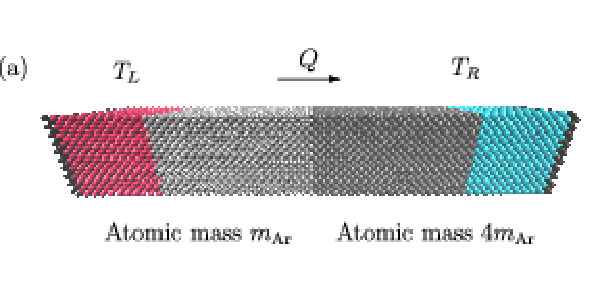
\includegraphics[width=.59\columnwidth]{inkscape/nemd_fig2a.pdf} 
  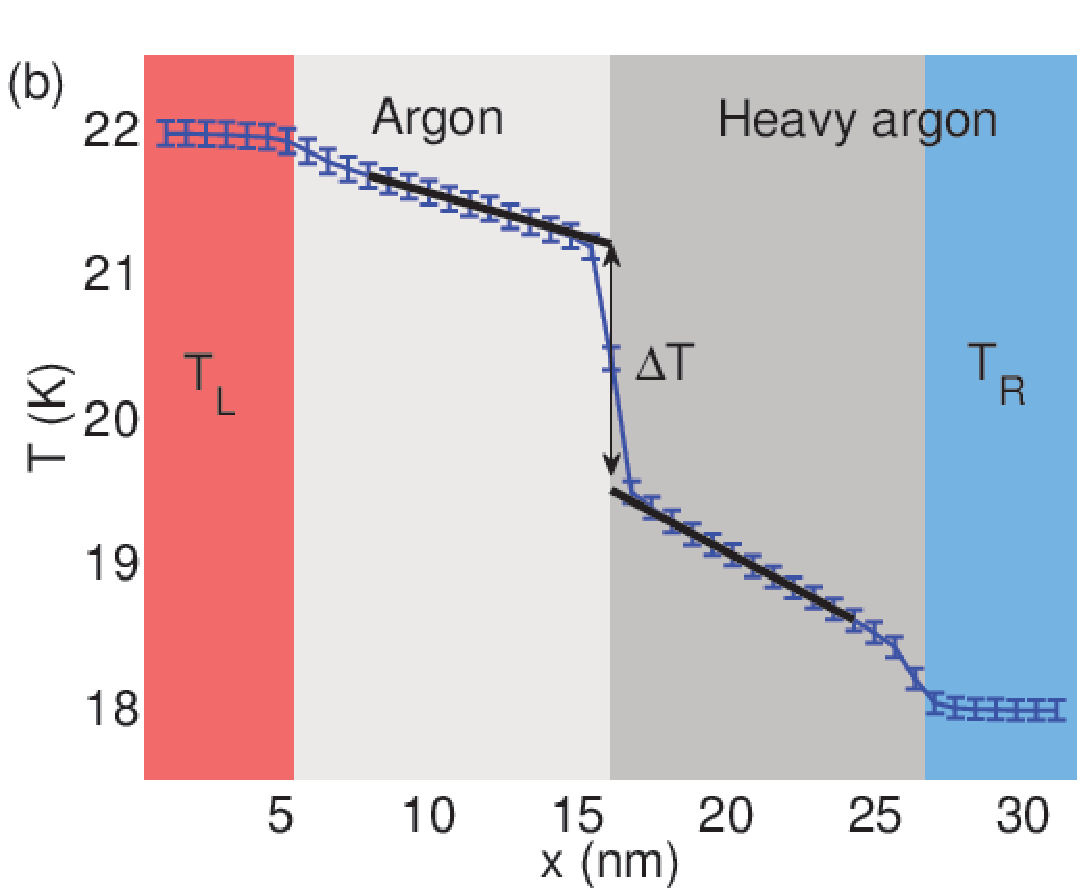
\includegraphics[width=.59\columnwidth]{inkscape/nemd_fig2b.pdf}
  \caption{(a) Simulation geometry used in \citepub{spectral} for investigating the role of anharmonic effects on vibrational energy transfer at mass-mismatched interfaces. (b) Steady-state temperature profile for a specific set of parameters. Reprinted with publisher's permission from \citepub{spectral}.}  
\label{fig:th_spectral_geom}
 \end{center}
\end{figure}

To outline the typical steps involved in a non-equilibrium simulation, consider the example setup of Fig. \ref{fig:th_spectral_geom}(a) used to investigate the anharmonic effects in interfacial heat transfer in \citepub{spectral}. In the setup of Fig. \ref{fig:th_spectral_geom}(a), the whole structure is first allowed to conform to zero-stress state by controlling atomic dynamics using a combination of a Nose-Hoover barostat and thermostat \cite{allentildesley}. Typical equilibration period consists of a few hundreds of thousands of time steps. After the initial equilibration, the size of the simulation box is fixed, and the positions of atoms located at the left- and right-most unit cells are frozen, preventing atomic sublimation at the free surfaces. Particles in the ''hot'' and ''cold'' regions, illustrated by the red and cyan coloured atoms in Fig. \ref{fig:th_spectral_geom}, are coupled to heat baths at temperatures $T_{\textrm{L}}$ and $T_{\textrm{R}}$ by including Langevin or Nos\'e-Hoover terms in their equations of motion. The system is then allowed to reach non-equilibrium steady state by integrating the equations of motion until the kinetic temperature profile shown in Fig. \ref{fig:th_spectral_geom}(b) and the heat current flowing through the system fluctuate around constant values. \change{The temperature profile of Fig. \ref{fig:th_spectral_geom}(b) is calculated by monitoring the atomic kinetic temperatures $T_i$ defined by the classical ''equipartition'' equation} \cite{allentildesley}
\begin{equation}
 \frac{1}{2} m_i \dot{\bb{x}}_i^2 = \frac{3}{2} k_B T_i.
\end{equation}
\change{The atomic temperatures $T_i$ are averaged temporally and also spatially by dividing the simulation domain into thin slabs and averaging over the atoms inside each slab}. 

After the steady state is reached, the simulation is continued typically for millions of time steps, and the values of observables such as temperature jump $\Delta T$ at the interface or the heat currents are determined from the trajectories. The statistical error in the determined quantities can be estimated by using standard methods described, e.g., in Ref. \cite{allentildesley}.

LAMMPS simulation package \cite{plimpton95} is used in Publications \cp{spectral}, \cp{cnt} and \cp{twinning} for integrating the equations of motion. The simulations of Publications \cp{fpu} and \cp{fpu2} are carried out using a house-made MD code. 

\section{Limitations of molecular dynamics and Green's function models}
\label{sec:th_limits}
MD and GF methods presented in the above sections are used in this thesis to investigate phononic energy transfer. Because MD is fully classical and therefore neglects all quantum effects, the method is strictly valid only at temperatures higher than the Debye temperature $T_D$ of the material under study\footnote{Debye temperature is defined here as $T_D=\hbar \omega_{max}/k_B$, where $\omega_{max}$ is the frequency of the highest-energy phonon mode.}. Despite this limitation, MD is still widely used and considered suitable \cite{cahill14} also at temperatures lower than $T_D$ due to its ability to capture the complex atomistic dynamics of solids, liquids, and gases, inherently including also non-linear effects through the anharmonic terms in the interatomic potential. 

\change{Another limitation of MD is that the classical force-fields used for describing interatomic forces are typically semi-empirical in nature and may not be transferable to arbitrary geometries. For example, the Stillinger-Weber potential \cite{stillinger85} used in} \citepub{twinning} \change{for describing Si-Si interactions is parameterized for bulk systems and may not therefore accurately capture atomistic dynamics at the nanowire surface. Such limitations could be partially removed by adopting more sophisticated force-fields such as the reactive force-field ReaxFF \cite{vanduin03} developed for large-scale chemistry simulations \cite{vanduin01} or by utilizing \textit{ab initio} MD \cite{car85}, where the instantaneous forces are extracted from density functional theory. While such methods are still prohibitively expensive for large-scale computer simulations, future improvements in computational power are expected to enable simulating energy transfer processes accurately in very complex systems including, e.g., biomolecules in a solvent. MD is therefore expected to keep providing powerful physical insight into the energy transfer processes taking place in nanosystems.}

% MD and GF methods presented in the above sections are used in this thesis to investigate phononic energy transfer. Because MD is fully classical and therefore neglects all quantum effects, the method is strictly valid only at temperatures higher than the Debye temperature $T_D$ of the material under study\footnote{Debye temperature is defined here as $T_D=\hbar \omega_{max}/k_B$, where $\omega_{max}$ is the frequency of the highest-energy phonon mode.}. \change{Something about the empirical potentials.} Despite this limitation, MD is still widely used and considered suitable \cite{cahill14} also at temperatures lower than $T_D$ due to its ability to capture the complex atomistic dynamics of solids, liquids, and gases, inherently including also non-linear effects through the anharmonic terms in the interatomic potential. MD can therefore deliver powerful physical insight into the energy transfer processes taking place in nanosystems.

In contrast to MD, the GF method fully captures quantum statistics. Being based on the algebraic solution of the linearized Langevin equations of motion, the method also straightforwardly delivers the spectrally decomposed thermal current [Eq. \eqref{eq:th_caroli}], which is only indirectly available from MD [Eq. \eqref{eq:th_spectral_curr}]. The drawback of the GF method is that it can only account for dissipative effects in terms of a single frequency-independent relaxation time given as an input parameter. The method is therefore not suitable for calculating, e.g., the thermal conductivity of materials. In addition, the method assumes small displacements of atoms from their equilibrium positions and cannot therefore be applied to the modeling of liquids, gases, or soft solids.

In addition to MD and GF methods, energy transfer in nanoscale can also be modeled using the Boltzmann transport equation \cite{ziman}. Boltzmann equation treats phonons as point-like particles and therefore neglects wave effects such as interference. The power of the method lies, however, in its applicability to large systems and its ability to straightforwardly capture various different scattering mechanisms in terms of phonon scattering rates calculated semi-empirically or from first principles methods. Recent advances in computational methods have allowed for a numerically exact solution of the Boltzmann equation in non-equi\-lib\-rium, enabling parameter-free determination of thermal conductivity \cite{broido07,ward09,lindsay13}. The applicability of the Boltzmann equation to the nanoscale structures considered in this thesis is, however, questionable due to its inability to capture interference effects, so only atomistic simulation methods are used in this thesis.
